% Project:			Mediation and Gender Differences
% This file:		Main writeup
% Original date: 	December 7, 2016

\documentclass[11pt]{article}

% colors
\usepackage[table]{xcolor}
\definecolor{maroon}{RGB}{153,0,18}
\definecolor{lime}{RGB}{190,213,88}
\definecolor{sand}{RGB}{217,202,179}
\definecolor{fire}{RGB}{144,50,61}
\definecolor{brick}{RGB}{94,11,21}
\definecolor{olive}{RGB}{117,109,84}
\definecolor{lavpink}{RGB}{172,123,132}
\definecolor{darkpurp}{RGB}{49,10,49}
\definecolor{salmon}{RGB}{204,90,113}
\definecolor{mauve}{RGB}{94,73,85}
\definecolor{greyblue}{RGB}{125,132,145}
\definecolor{greypurp}{RGB}{68,56,80}
\definecolor{brightpurp}{RGB}{96,20,255}

% packages (please add in alphabetical order)
\usepackage{adjustbox}
\usepackage{amsfonts}
\usepackage{amsmath}
\usepackage{amssymb}
\usepackage{array}
\usepackage{bm}
\usepackage{booktabs}
\usepackage{caption}
\usepackage{epstopdf}
\usepackage{float}
\usepackage[margin=1in]{geometry}
\usepackage{graphicx}
\usepackage[colorlinks=true, linkcolor=brightpurp, citecolor=brightpurp, urlcolor=salmon]{hyperref}
\usepackage{lipsum}
\usepackage{longtable}
\usepackage{mathtools}
\usepackage{multirow}
\usepackage{natbib}
\usepackage{rotating}
\usepackage{setspace}
\usepackage{subcaption}
%\usepackage{threeparttable}
\usepackage{threeparttablex}
\usepackage{xr}
\usepackage[printwatermark]{xwatermark}


\newcolumntype{L}[1]{>{\raggedright\let\newline\\\arraybackslash\hspace{0pt}}m{#1}}
\newcolumntype{C}[1]{>{\centering\let\newline\\\arraybackslash\hspace{0pt}}m{#1}}
\newcolumntype{R}[1]{>{\raggedleft\let\newline\\\arraybackslash\hspace{0pt}}m{#1}}

% commands
\newcommand{\mr}{\multirow}
\newcommand{\mc}{\multicolumn}


\externaldocument{mediation-gd_appendix}

\begin{document}


\title{Gender Differences in the Effects of Early Childhood Education}
\author{Jorge Luis Garc\'{i}a \and James J. Heckman \and Anna L. Ziff}
\date{Original date: December 7, 2016 \\ Current date: \today}
\maketitle

\section{Proposed Outline}

\begin{enumerate}
\item	Introduction
	\begin{enumerate}
		\item There are gender differences in the current economy. These are especially pronounced when considering disadvantage as well.
		\item Previous studies have shown the efficiency of investing early in life, especially for children from disadvantaged families
		\item How are these later-life differences mediated by early life experiences?
	\end{enumerate}
\item Program
	\begin{enumerate}
		\item Description of ABC/CARE intervention and study
		\item Description of data collection points and measures collected
	\end{enumerate}
\item Treatment Effects
	\begin{enumerate}
		\item Tables with treatment effects on inputs and outputs
		\item More in depth description of parenting measures and select outcomes (crime)
	\end{enumerate}
\item Mediation
	\begin{enumerate}
		\item Early skills on later skills
		\item Later skills on adult mediators (education)
		\item Adult mediators on outcomes of interest (income)
	\end{enumerate}
\item Conclusion
\end{enumerate}

%\input{sections/abstract}
\tableofcontents

\doublespacing

\section{Introduction}
\label{sec:introduction}
\input{sections/introduction}	

\section{Data}
\label{sec:data}
\subsection{Data Sources} \label{section:data}
\noindent FAM uses data from ABC/CARE follow-up surveys to set the initial state of the cohort.
The transition model parameters are estimated from the 1997 to 2013 waves of the Panel Study of Income Dynamics (PSID).
We supplement the PSID with data from the Health and Retirement Study (HRS). We use the National Health and Nutrition Examination Survey (NHANES)
to account for differences between measured and self-reported BMI.
To estimate medical care costs associated with health conditions, we use the Medical Expenditures Panel Survey (MEPS) and the Medicare Current Beneficiaries Survey (MCBS).


\subsubsection{PSID}
\label{section:data_psid}
%The Panel Survey of Income Dynamics (PSID) is a longitudinal household survey containing between 5,000 and 8,500 families in each wave, which began yearly in 1968 and is fielded biennially since 1996. When appropriately weighted, the PSID is designed to be representative of U.S. households. The PSID provides extensive information concerning demographics, economic outcomes, health care access, health outcomes, and health behaviors (such as smoking history, alcohol consumption, and exercise habits). Health outcome variables include diagnosis of diabetes, heart disease, hypertension, lung disease, cancer, etc.

\noindent The Panel Study of Income Dynamics (PSID) provides extensive information concerning demographics, economic outcomes, health care access, health outcomes, and health behaviors (such as smoking history, alcohol consumption, and exercise habits). Health outcome variables include diagnosis of diabetes, heart disease, hypertension, lung disease, and cancer, among others.

\noindent We estimate the transition models using waves from 1997 to 2013. We create a dataset of respondents who have formed their own households, either
as single heads of households, cohabiting partners, or married partners. These heads, wives, and husbands respond to the richest
set of PSID questions, including the health questions that are critical for our purposes. We use all respondents aged 25 and older.\footnote{While we use the full sample in our main analysis, we explored using a few different subsamples to better adapt to the demographics of the ABC/CARE subjects.}
The length of the PSID is a significant advantage, because we can include past health behaviors as explanatory variables for current health outcomes. This dataset provides adequate sample sizes to explore health outcomes of specific groups.
PSID does not follow individuals who are institutionalized in nursing homes or other long-term care facilities. To overcome this weakness, we pool the PSID sample with the HRS sample when
estimating mortality models.

\subsubsection{HRS}

\noindent The Health and Retirement Study (HRS) is a longitudinal panel that surveys a nationally representative sample of individuals over the age of 50 and their spouses every two years. When appropriately weighted, the HRS in 2010 is representative of U.S. households
where at least one member is at least 51 years old.
This study collects in-depth information about income, work, health, and medical expenditures. In our model, waves from 1998 to 2012 are pooled with the PSID for estimation of mortality and
widowhood models. The HRS data
are harmonized to the PSID for all relevant variables. Because the PSID does not follow respondents into nursing homes, we also use the HRS to estimate the model for nursing home residency. We use all cohorts in the dataset created by RAND (RAND HRS, version O) as the basis
for our analysis.

\subsubsection{MCBS}
\noindent The Medicare Current Beneficiary Survey (MCBS) is a nationally representative sample of aged, disabled,
and institutionalized Medicare beneficiaries. The MCBS attempts to interview each respondent twelve
times over three years, regardless of whether he or she resides in the community, a facility, or
transitions between community and facility settings. The disabled (under 65 years of age) and
very elderly (85 years of age or older) are over-sampled. The first round of interviewing was conducted
in 1991. Originally, the survey was a longitudinal sample with periodic supplements and indefinite
periods of participation. In 1994, the MCBS switched to a rotating panel design with limited periods
of participation. Each fall, a new panel is introduced, with a target sample size of 12,000 respondents. Each summer, a panel is retired. Institutionalized respondents are interviewed by proxy. The MCBS
contains comprehensive self-reported information on the health status, health care use and
expenditures, health insurance coverage, and socioeconomic and demographic characteristics of the
entire spectrum of Medicare beneficiaries. Medicare claims data for beneficiaries enrolled in
fee-for-service plans are also used to provide more accurate information on health care use and
expenditures. MCBS data from 2007 to 2010 are used for estimating medical costs and enrollment models.

\subsubsection{MEPS}
\noindent The Medical Expenditure Panel Survey (MEPS), which began in 1996, is a set of large-scale surveys of families and individuals, their medical providers, and employers across the U.S. The Household Component (HC) of the MEPS provides data from
individual households and their members, which is supplemented by data from their medical providers.
The HC collects data from a representative subsample of households drawn from the
previous year's National Health Interview Survey (NHIS). Since NHIS does not include the
institutionalized population, neither does MEPS; this implies that we can only use the MEPS to
estimate medical costs for the non-elderly (ages 25--64) population. Information collected during household
interviews include: demographic characteristics, health conditions, health status, use of medical
services, sources of medical payments, and body weight and height. Each year the household survey
includes approximately 12,000 households, or 34,000 individuals. Sample size for those aged 25-64 is
about 15,800 in each year. MEPS has comparable measures of socioeconomic status as those in PSID,
including age, race and ethnicity, educational attainment, census region, and marital status. We estimate medical expenditure
and utilization using data from 2008 to 2010. We use waves from 2001 to 2003 to estimate models of quality-adjusted life years (QALYs), due to availability of EQ-5D instrument in these waves.\footnote{Section \ref{section:FAM_models} explains the estimation of the QALY model.}


\subsubsection{NHANES}
\noindent
The National Health and Nutrition Examination Survey (NHANES) targets a nationally representative sample of approximately 5,000 individuals in each year since 1999. The data collected includes responses to interview questions about demographics, disease conditions, height, and weight, as well as physical measurement of BMI. We use NHANES years 2002 to 2010 to estimate a model for imputing measured BMI from self-reported BMI. The methodology is described in Section \ref{section:FAM_ABC_impute}.

\subsubsection{ABC/CARE}
\noindent FAM uses ABC/CARE data to initialize the state of each ABC/CARE subject when they enter into the simulation.
These data are taken from the the parental interviews at various subject ages from birth to age 21; age-30 subject interview; and mid-30s biomedical survey.
The goal is to have each subject's initial state in the simulation match their status at the age-30 subject interview. However, because several key FAM inputs are not available at the age-30 interview, we use PSID or ABC/CARE surveys corresponding to other ages to impute missing elements. These imputations are discussed in Section \ref{section:FAM_ABC_impute}.

\paragraph{Variable Construction and Imputations}
\label{section:FAM_ABC_impute}

% \todo would be nice to have a table that summarizes imputed variables at age 30, imputation method, and number of missing subjects

\noindent Marital status transitions and childbearing in FAM are affected by the subject's mother's education level. The ABC/CARE age-30 subject interview did not ask about mother's education, but the ABC age-21 parent interview did.
For ABC subjects, we assume that each subject's mother had the same education level at the age-30 subject interview as what was reported in the age-21 parent interview. For CARE subjects, we impute mother's education from an ordered Probit model using race, ethnicity, education, disease conditions, employment status, presence of a health-related work limitation, and a self-report of whether or not the subject was ``poor'' as a child.  The model is estimated using age 30 to 31 PSID subjects with birth years between 1945 and 1981. Each of the model covariate values are taken from the CARE age 30 interview. At the beginning of each simulation repetition, an education level is randomly drawn from the probability distribution for each CARE subject and assigned to be the mother's education level.

\noindent Many FAM transition models depend on a three-level measure of parents' economic status when the subject was a child.
This is based on the PSID question: ``Were your parents poor when you were growing up, pretty well off, or what?''
The three possible responses are ``poor,'' ``average''/``it varied'', or ``pretty well off.''
This question is not included in the ABC/CARE interviews, but because preliminary eligibility for the program focused on children from high-risk backgrounds, based on socioeconomic factors, the value of this variable is set to ``poor'' (when growing up) for all ABC/CARE subjects.

\noindent All FAM transition models depend on demographics of the subject, including whether or not the subject is Hispanic.
This information is not available in the ABC/CARE data, but it is assumed that none of the ABC/CARE subjects are Hispanic.\footnote{Census data on Hispanics in North Carolina were not available for 1970 and 1980, but Hispanic migration into this state is more recent than in other regions, and as late as 1990, only 2\% of the North Carolina poor were Hispanic \citep{Johnson_2003_Changing-Poverty}.}

\noindent Most FAM models depend on smoking status. Employment status affects FAM transitions in marital status, childbearing, claiming of disability insurance (DI) and supplemental security income (SSI), and type of health insurance.
One male in the ABC control group is missing smoking status and, although known to be not working, is also missing specific employment status (unemployed or out of the labor force).
 We use a multinomial logit model to jointly estimate the probability of each combined smoking and employment category among 25- to 35-year-olds in the PSID who were not working. At the beginning of each simulation repetition, we use a Monte Carlo random draw generated from this distribution to assign this subject's smoking and employment statuses. This same subject is also missing information about binge drinking. A separate binary Probit binge drinking model was estimated using the age 25--35 PSID data. A Monte Carlo random draw is taken according the Probit probability to forecast binge drinking behavior at the beginning of the simulation.

\noindent BMI affects FAM transitions in health, functional status, employment, and smoking.
The FAM transition models are estimated with BMI computed from self-reported height and weight in the PSID.
The only BMI data in ABC/CARE come from height and weight measured during the health interview. This interview took place at roughly age 30 for CARE subjects, and at age 34 for ABC subjects.
This poses two challenges.
First, self-reported BMI can be biased by factors such as actual height and weight, gender, and race.\footnote{\citet{Cawley_2004_JHR}.}
Second, it is possible that BMI could increase or decrease systematically in the years between the age-30 subject interview and the age-34 health interview.

\noindent To address the first BMI imputation challenge, we use a variation on the method of \citet*{Courtemanche_etal_2015_Adjusting-Body-Mass} to impute measured BMI in the PSID.
While the method in \citet{Courtemanche_etal_2015_Adjusting-Body-Mass} works for importing height and weight, we apply the following specification to directly model BMI. Using respondents aged 30 to 40 in the 2002-2010 NHANES waves, we forecast measured BMI from percentile ranks of self-reported BMI using the model specification in \citet{Courtemanche_etal_2015_Adjusting-Body-Mass}. Three variations
on the spline interactions of \citet{Courtemanche_etal_2015_Adjusting-Body-Mass} are also considered. After estimating these models using NHANES data, covariate values from the PSID
age 30--34 data in years 2002--2013 are used to impute measured BMI values for PSID respondents. A Kolmogorov-Sminov (K-S) test and a visual inspection of smoothed histograms are used to compare the distribution of PSID imputed values to the distribution of observed values in the NHANES estimation sample. The model specification used for imputation has the smallest K-S distance between the two distributions.

\noindent After imputing values of measured BMI for PSID respondents age 30--34, we turn to the second problem: accounting for systematic trends in BMI from the age 30 interview to the health interview. The goal is to have a model that maps from measured BMI at the health interview around age 34 to self-reported BMI at the age 30 interview. Employing the longitudinal structure of PSID, we match each respondent's first interview between age 30--32 with their imputed measured BMI between ages 33--40. We then estimate a model using self-reported BMI between ages 30--32 as the response variable and imputed measured BMI at ages 33--40, the age when BMI is actually measured, along with other variables observed at age 30 as explanatory variables. This imputation model is applied to any ABC/CARE subject who has their health interview at least one year after their age 30 interview.

\noindent For ABC/CARE subjects who have their health interview within one year of the age 30 interview, we assume that any systematic time trends in BMI are too small to have any practical significance. However, we still need to convert the imputed measured BMI to a self-reported value for compatibility with other transition models estimated in PSID. This model is estimated on ages 30--32 in the PSID and uses covariates from the age 30 interview along with imputed measured BMI to forecast self-reported BMI.

\noindent At the beginning of each simulation repetition, we choose the appropriate model to impute self-reported BMI for each ABC/CARE subject based on the time between their age 30 interview and their health interview. Their expected BMI is estimated from this model. A Monte Carlo Normal random draw is generated using the subject's expected BMI and the estimated variance from the model. This Monte Carlo draw is then assigned to be the subject's initial self-reported BMI in the simulation. Using BMI from the health interview limits the ABC/CARE subjects simulated in FAM to only those who have height and weight measurements in the health interview.

\noindent Subjects' health insurance coverage affects their medical costs.
FAM uses three categories of health insurance: none, public only, and some private.
Five ABC subjects and three CARE subjects were missing health insurance status.
Three cases were logically imputed by assuming that subjects have no health insurance if they do not know their insurance status and either go to an emergency room or community health clinic or do not go anywhere when they need health care.
In order to impute the insurance category for the remaining five cases, we use age 25--35 PSID data to estimate a Probit model for whether or not a subject had insurance.
The predictors were gender, earnings, marital status, self-reported health, employment status, and whether or not the subject had any biological children.
We use this model to compute the probability of having insurance at the start of the simulation (at the age-30 interview).
Then, we generate a Monte Carlo binary random variate according to this probability.
If the outcome is positive, the subject is assigned to have some private insurance.

\noindent FAM uses six Activities of Daily Living (ADLs) about which there is data in PSID: walking, dressing, eating, bathing or showering, getting in and out of bed or a chair, and using the toilet, including getting to the toilet.
FAM simulates the number of these ADLs in which the subject has difficulty.
ADL difficulties forecast FAM transitions in benefits claiming, mortality, employment status, insurance category, and nursing home residency.
FAM also transitions the count of difficulties among six Instrumental Activities of Daily Living (IADLs) from PSID: preparing one's own meals; shopping for personal toilet items or medicines; managing one's own money, such as keeping track of expenses or paying bills; using the phone; doing heavy housework, like scrubbing floors or washing windows; and doing light housework, like doing dishes, straightening up, or light housecleaning.
Both ADLs and IADLs are components of FAM's model for quality-adjusted life years (QALYs).
The ABC/CARE age-30 subject interview does not ask about ADLs or IADLs, but it does ask if the subject has a physical or nervous condition that keeps them from working.
PSID respondents are also asked this question.
We create an imputation model for each of these two measures using an ordered Probit model estimated on PSID respondents aged 25 to 35.
We use these models to compute the probabilities for each number of ADLs and IADLs. To start the simulation, we generate Monte Carlo random draws according to these probabilities and use them to assign the corresponding counts.

\noindent When a subject claims DI benefits, it affects their FAM transitions in employment status, insurance category, and Medicare enrollment.
DI claiming also affects medical costs.
SSI claiming affects FAM transitions in employment status.
Lastly, claiming Social Security retirement benefits affects FAM transitions in employment status and insurance category.
The ABC age-30 subject interview has a single yes/no question about claiming which asks: ``Currently are you receiving income from workman's compensation, disability, or Social Security benefits including Supplemental Security Income?'' CARE asks a similar question. The PSID has separate questions for each benefit type. We use a multinomial logit model to estimate the joint probability of each combination of DI and SSI claiming. The estimation uses PSID respondents aged 25 to 35 who were claiming at least one of the following benefits: workman's compensation, DI, or SSI. A Monte Carlo random draw generated from this distribution is used to assign each ABC/CARE subject's DI- and SSI-claiming status at the start of the simulation. One ABC subject is missing data about whether or not they were claiming and was assumed to not be claiming any benefits.

\noindent As discussed in Section \ref{section:FAM_models}, FAM uses different models to estimate medical costs depending on whether or not a subject is Medicare-eligible. Subjects can enroll in Medicare before the age of 65 if they are claiming DI. The cost estimates for Medicare-eligible subjects depend on the subjects' current disease status at the age-30 interview and their disease status two years prior to the interview. Unfortunately, ABC/CARE does not have disease data two years before the age-30 interview. It is assumed that all subjects do not have their disease conditions in the previous period.










% \todo we could add a table of all the FAM input variables (rows) and three columns, as-is, rule imputed, model imputed, with checkmarks to indicate how the data were derived
	

\section{Gender Differences}
\label{sec:gdiff}
We present a summary of the difference in treatment effects between males and females. For each outcome, $Y$, we estimate  Equation~\eqref{eq:te}, which accounts for the levels of the treatment effect and the ``male'' effect,

\begin{equation}
\label{eq:te}
Y = \beta_0 + \beta_1 [\text{treatment}] + \beta_2 [\text{male}] + \beta_3 [\text{treatment} \times \text{male}] + \beta X + \varepsilon.
\end{equation}

\noindent Assuming that $\varepsilon$ is a mean-zero and conditionally independent disturbance, the estimated $\beta_3$ reveals the gender difference of the treatment effect.

We group the outcomes by broad, life-relevant categories and code the outcomes such that $\beta_1 > 0$ indicates a more socially positive treatment effect. We resample with replacement 100 times. In each bootstrap, we calculate, by category, the proportion of variables for which the gender differences ($\beta_3$) is negative. A negative gender difference indicates that the treatment has a more socially positive effect on females than on males after controlling for the treatment effect, the male effect, and background variables unaffected by treatment.\footnote{These background variables are mother's IQ and mother's years of education when the subject was born.}

As seen in Appendix~\ref{app:data}, measures of IQ and achievement are internally consistent within and across time periods. This is not always the case for social-emotional skills. We leverage the consistency of the cognitive measures to create additional measures of achievement net of IQ. This captures the skill measured by achievement scores orthogonal to that measured by IQ scores.

Figure~\ref{fig:prop-category} shows, for each category, the proportion of variables with negative gender differences ($\beta_3 < 0$, females $>$ males). When aggregating all outcomes, the gender differences are not apparent: 54.2\% of all gender differences are negative, but this is not statistically different from the null hypothesis of 50\%. However, dividing the variables by category shows considerable gender differences. Females have more positive effects on achievement and social-emotional scores, using both traditional social-emotional batteries and the social-emotional construct described above. Treatment also more positively affected them when considering labor market outcomes (including education, employment, and income) and crime outcomes. Consistent with other studies, males benefit more in health outcomes.\footnote{\citet{Campbell_Conti_etal_2014_EarlyChildhoodInvestments,Conti_etal_2016_LongTermHealth}.}

\begin{figure}[H]
\begin{center}
\caption{Proportion of Outcomes with Negative Gender Difference by Category}
\label{fig:prop-category}
\includegraphics[width=\textwidth]{../output/abccare-counts-category}
\end{center}
\raggedright \footnotesize
Note: Each category is comprised of related variables. All variables are coded such that higher values correspond to socially positive outcomes. Teen Ach. net IQ is achievement at ages 12 and 15 net of IQ. Late Ach. net IQ is the same but for achievement at age 21. Labor and Parent include education, employment, and income variables for the subject and parent, respectively. 
\end{figure}

\begin{table}[H]
\centering
\caption{Treatment Effects, Parenting Skills}
\label{te-parenting}
\begin{adjustbox}{width=\textwidth}
\begin{threeparttable}
	\input{../output/abccare-parenting}
\begin{tablenotes}
\item Note: This table displays the treatment effects 
\end{tablenotes}
\end{threeparttable}
\end{adjustbox}
\end{table}

\begin{table}[H]
\centering
\caption{Treatment Effects, Cognitive Skills}
\label{te-cognitive}
\begin{adjustbox}{width=\textwidth}
\begin{threeparttable}
	\input{../output/abccare-cognitive}
\begin{tablenotes}
\item Note:
\end{tablenotes}
\end{threeparttable}
\end{adjustbox}
\end{table}

\begin{table}[H]
\centering
\caption{Treatment Effects, Non-cognitive Skills}
\label{te-ncognitive}
\begin{adjustbox}{width=\textwidth}
\begin{threeparttable}
	\input{../output/abccare-ncognitive}
\begin{tablenotes}
\item Note:
\end{tablenotes}
\end{threeparttable}
\end{adjustbox}
\end{table}

\begin{table}[H]
\centering
\caption{Treatment Effects, Education}
\label{te-education}
\begin{adjustbox}{width=\textwidth}
\begin{threeparttable}
	\input{../output/abccare-education}
\begin{tablenotes}
\item Note:
\end{tablenotes}
\end{threeparttable}
\end{adjustbox}
\end{table}


\subsection{Inputs}

We explore the effects of the intervention on parenting in more detail. This allows us to understand the gender differences of this important input. We use measurements of the Home Observation for Measurement of the Environment (HOME; \citet{Bradley-Caldwell_1977_AJMD}), which measures the quality of the child's home environment.\footnote{Although the exact scales vary by age, the subscales of the HOME measure generally measure maternal warmth and involvement, absence of punishment, provision of appropriate toys, encouragement of mature behavior and independence, and the physical and language environment. The full score is the sum of these subscales.}

When graphing the density of a factor combining the full HOME scores measured at different ages, the density of the treatment group in both the male and female subsamples is bimodal (Figure~\ref{fig:total-home}). Because this is not the case for the control group, it is possible that treatment is moderated by another input of home environment. We consider the input of father's presence. For males, the mean of the treatment group if the father is present is greater than that of the treatment group if the father is absent. The reverse is seen for the females. 

\begin{figure}
\begin{center}
\caption{Density of the HOME Scores by Gender and Experimental Group}
\label{fig:total-home}

	\begin{subfigure}[b]{0.49\textwidth}
		\centering
		\caption{Factor HOME Scores, Males}
		\label{fig:home-male-factor}
			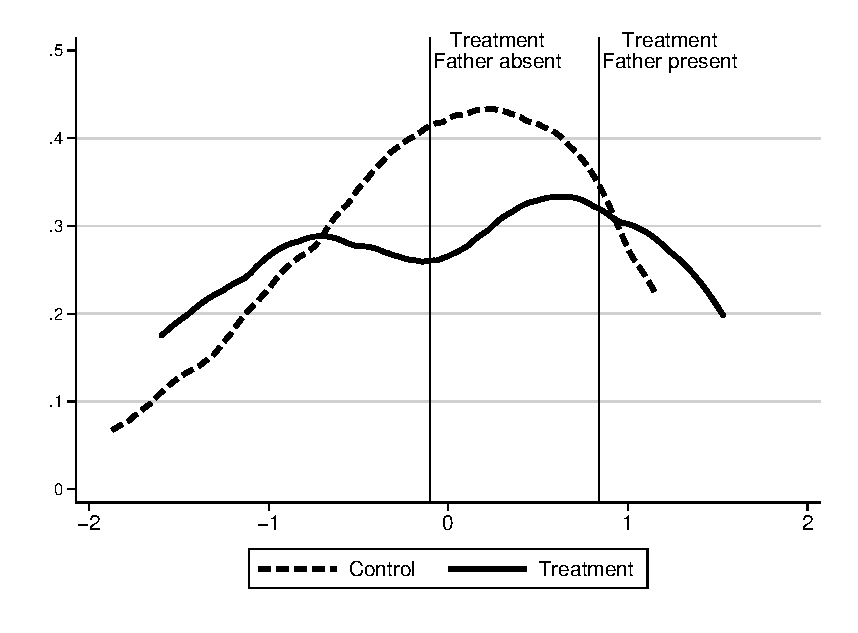
\includegraphics[width=\textwidth]{../output/HOME-males-factorhome}
	\end{subfigure}
	\begin{subfigure}[b]{0.49\textwidth}
		\centering
		\caption{Factor HOME Scores, Females}
		\label{fig:home-female-factor}
			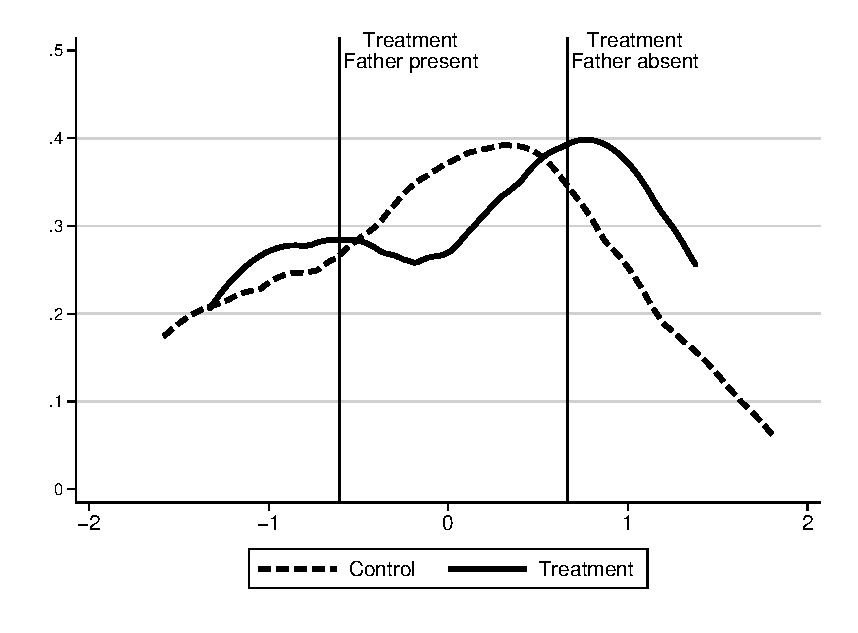
\includegraphics[width=\textwidth]{../output/HOME-females-factorhome}
	\end{subfigure}
\end{center}
\raggedright
Note: These plots show the distribution the factor of HOME scores. The factors are computed by gender using full HOME scores at 0.5, 1.5, 2.5, and 8 years. The vertical lines are the means of the treatment group by father's presence. 
\end{figure}

We explore this trend more closely in Figure~\ref{fig:total-home-quantiles}. To do so, we calculate the distribution pooling experimental groups but splitting by gender and father's presence. We then calculate, by gender and father's presence, the proportion of the treatment group that is in quantile 1 versus quantile 2. We do the same for the control group. 

The result of this exercise shows that the bimodal shape of the densities of the treatment group is explained differently by gender. For males, the HOME scores are higher for the control group when the fathers are absent and higher for the treatment group when father's are present. For females, the opposite is the case: The HOME scores are higher for the control group when fathers are present and higher for the treatment group when fathers are absent. 

One explanation of this is that treatment complements father's presence for males but substitutes it for females. Mothers then compensate for the father's absence for males (females) in the control (treatment) group. 

%One way mothers can compensate for the father's absence for males is to enroll them in alternate preschool arrangements. This is seen with more males in the control group being enrolled in these arrangements than control-group females (Figure~\ref{fig:alt-enrollment}). 

\begin{sidewaysfigure}
\begin{center}
\caption{Factor HOME Scores}
\label{fig:total-home-quantiles}
	\begin{subfigure}[b]{0.49\textwidth}
		\centering
		\caption{HOME, Father Absent, Males}
		\label{fig:home-male-mean}
			\includegraphics[width=\textwidth]{../output/HOME-male1-fhome0-2quant}
	\end{subfigure}
	\begin{subfigure}[b]{0.49\textwidth}
		\centering
		\caption{HOME, Father Absent, Females}
		\label{fig:home-female-mean}
			\includegraphics[width=\textwidth]{../output/HOME-male0-fhome0-2quant}
	\end{subfigure}
	
	\begin{subfigure}[b]{0.49\textwidth}
		\centering
		\caption{HOME, Father Present, Males}
		\label{fig:home-male-factor}
			\includegraphics[width=\textwidth]{../output/HOME-male1-fhome1-2quant}
	\end{subfigure}
	\begin{subfigure}[b]{0.49\textwidth}
		\centering
		\caption{HOME, Father Present, Females}
		\label{fig:home-female-factor}
			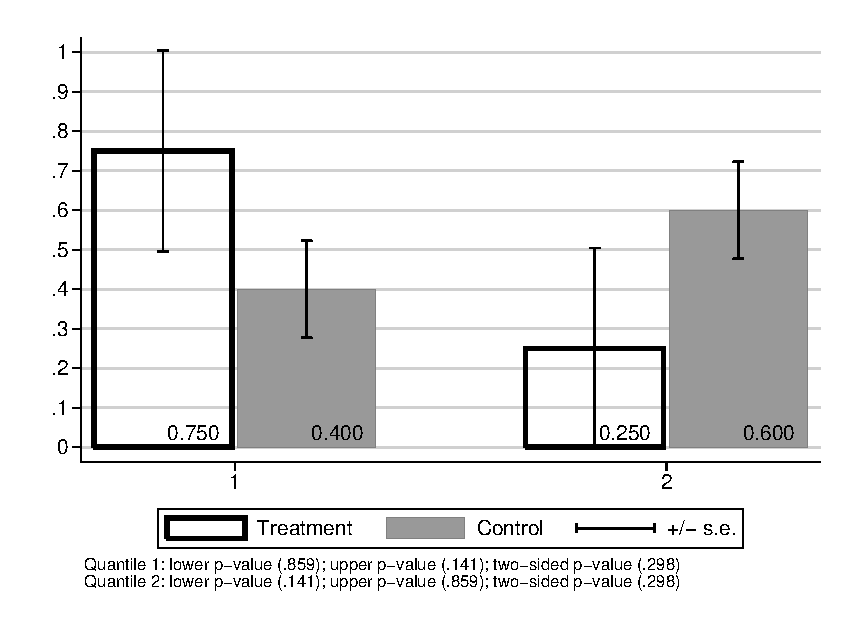
\includegraphics[width=\textwidth]{../output/HOME-male0-fhome1-2quant}
	\end{subfigure}
\end{center}
\raggedright \footnotesize
Note: The horizontal axis divides a factor of the HOME scores into the first and second quantile of the distribution pooling across experimental groups, but splitting  by gender and father's presence. The factors are computed by gender using full HOME scores at 0.5, 1.5, 2.5, and 8 years. The lower $p$-value tests that the treatment proportion is less than the control proportion within a quantile. The upper $p$-value tests that the treatment proportion is greater than the control proportion within a quantile. The numbers reported in the bars are the proportions. All standard errors and $p$-values are calculated using 1,000 bootstraps.
\end{sidewaysfigure}

%\begin{figure}
%\begin{center}
%\caption{Alternate Preschool Enrollment}
%\label{fig:alt-enrollment}
%	\begin{subfigure}[b]{0.49\textwidth}
%		\centering
%		\caption{Males by Father's Presence}
%			\includegraphics[width=\textwidth]{../output/family-dcmopre-father-male}
%	\end{subfigure}
%	\begin{subfigure}[b]{0.49\textwidth}
%		\centering
%		\caption{Females by Father's Presence}
%			\includegraphics[width=\textwidth]{../output/family-dcmopre-father-female}
%	\end{subfigure}
%	
%		\begin{subfigure}[b]{0.49\textwidth}
%		\centering
%		\caption{Pooled}
%			\includegraphics[width=\textwidth]{../output/family-dcmopre}
%	\end{subfigure}
%	\end{center}
%\raggedright
%Note: These histograms display the distributions of the months of enrollment in alternative preschool by gender. Months of enrollment are cumulative between birth and 5 years. 
%\end{figure}

\subsection{Adult Outcomes}

\begin{figure}[H]
\begin{center}
\caption{Crime}
\label{fig:}	
	\begin{subfigure}[b]{0.49\textwidth}
		\centering
		\caption{Felonies}
			\includegraphics[width=\textwidth]{../output/Outcomes_Correlation/abccare/crime/bar-gender-trt-ad34_fel}
		\end{subfigure}
	\begin{subfigure}[b]{0.49\textwidth}
		\centering
		\caption{Misdemeanors}
			\includegraphics[width=\textwidth]{../output/Outcomes_Correlation/abccare/crime/bar-gender-trt-ad34_mis}
	\end{subfigure}
	\end{center}
\raggedright \footnotesize
Note:
\end{figure}

\begin{figure}[H]
\begin{center}
\caption{Age of First Crime}
\label{fig:age-first-crime}
	\includegraphics[width=\textwidth]{../output/Outcomes_Correlation/abccare/crime/bar-gender-trt-juv_crime_age}
\end{center}
\raggedright \footnotesize
Note:
\end{figure}		

\section{Mediation Analysis}
\label{sec:results}
To find a set of early, school-age, and adult mediators, we start by focusing on two life-cycle outcomes: labor income and savings in crime costs, both of which are in net present value of 2014 dollars discounted to birth of the subjects assuming a 3\% discount rate.\footnote{These outcomes are estimated following the methods described in \citet{Garcia_etal_2016_Comp_CBA_Unpublished}. These outcomes allow us to analyze the mediation beyond the ages observed at data collection. The inference for the following analysis accounts for the construction of the net present value of income, which uses an auxiliary sample to predict unobserved earnings. We bootstrap over the auxiliary sample in addition to bootstrapping over the ABC/CARE sample. The auxiliary data for crime is the complete population of individuals who committed crimes in North Carolina.}

We first estimate the effect of the early mediators, $\bm{\theta^E}$, on the school-age mediators, $\bm{\theta^S}$. In this case, $\bm{\theta^E}$ and $\bm{\theta^S}$ are vectors containing cognitive, non-cognitive, and parenting skills. For each $\theta^E_s$ in $\bm{\theta^S}$, we calculate

\begin{equation}
	\theta^S_s = \alpha_0 +\bm{ \alpha} \bm{\theta^E} + \varepsilon.
\end{equation}

Then, we estimate the effect of the school-age mediators on the adult mediators, $\bm{\theta^A}$. For each $\theta^A_a$ in $\bm{\theta^A}$, we calculate:

\begin{equation}
	\theta^A_a = \mu_0 + \bm{\mu} \bm{\theta^S} + \epsilon.
\end{equation}

Finally, we estimate the effect of the later mediators on the outcome of interest, $Y$:

\begin{equation}
	Y = \gamma_0 +\bm{\gamma} \bm{\theta^A} + \nu. 
\end{equation}

All of the parameters in these equations are estimated in the full sample of ABC/CARE. That is, we impose that the technology is the same across genders. We then split the sample by gender to calculate the treatment effect and decompose it based on the inputs of the above equations. To get the proportions reported below, we multiply this treatment effect by the estimates of the corresponding parameters from the above equations, and divide by the total treatment effect. This is a standard Laspeyres decomposition.

A pattern that emerges when considering the early and school-age skills as mediators is that cognitive skills tend to mediate for females more so than for males, and that the reverse is true for non-cognitive and parenting skills.

\begin{figure}[H]
\begin{center}
\caption{Early Skills on School-age Non-cognitive Skills}
\label{fig:earlyskills-ncog}
	\includegraphics[width=\textwidth]{../output/mediation/ncogfactor-nch-1-1-1}
\end{center}
\raggedright
Note: 
\end{figure}


\begin{figure}[H]
\begin{center}
\caption{Early Skills on School-age Retention}
\label{fig:earlyskills-retention}
	\includegraphics[width=\textwidth]{../output/mediation/never_ret-nch-1-1-1}
\end{center}
\raggedright
Note: 
\end{figure}


\begin{figure}[H]
\begin{center}
\caption{School-age Skills on Years of Education}
\label{fig:schoolskills-years}
	\includegraphics[width=\textwidth]{../output/mediation/years_30y-ncr-1-1-1}
\end{center}
\raggedright
Note: 
\end{figure}


\begin{figure}[H]
\begin{center}
\caption{School-age Skills on College Graduation}
\label{fig:schoolskills-univ}
	\includegraphics[width=\textwidth]{../output/mediation/si30y_univ_comp-ncr-1-1-1}
\end{center}
\raggedright
Note: 
\end{figure}

\begin{figure}[H]
\begin{center}
\caption{High School Graduation on Lifetime Income}
\label{fig:hs-npvincome}
	\includegraphics[width=\textwidth]{../output/mediation/income-s-1-1-1}
\end{center}
\raggedright
Note: 
\end{figure}

\begin{figure}[H]
\begin{center}
\caption{High School Graduation on Lifetime Crime Savings}
\label{fig:hs-npvcrime}
	\includegraphics[width=\textwidth]{../output/mediation/crime-s-1-1-1}
\end{center}
\raggedright
Note: 
\end{figure}


%\section{Summary}
%\label{sec:conclusion}
%When considering the early and school-age skills mediating educational attainment, we find that non-cognitive skills are significant mediators for both males and females. Given the importance of educational attainment in mediating other adult outcomes, the fact that non-cognitive skills are mediators for it highlights the dynamic importance of the non-cognitive skills. 
The proportion of the treatment effect explained by the skills do not differ by gender. Instead, the treatment effects for years of education are much larger for females than for males. 

Gender differences also appear when considering educational attainment as a mediator for labor income. At age 30, years of education is a negative mediator of labor income for females. This indicates that more educated women are staying at home, i.e., although treatment may increase years of education, that in turn does not necessarily lead to a full-time career by age 30. However, when considering the lifetime income, we find that the educational attainment has the opposite effect. In this case, educational attainment for females positively mediates labor income. It is striking to compare these results to those of the males, in which educational attainment is not a significant mediator income for neither the age-30 nor the lifetime income. Although females may exit the labor force during their child-bearing years, they re-enter and recover income through their increased educational attainment. 

Finally, we consider crime savings to explore another way in which educational attainment can mediate the adult treatment effects. For females, years of schooling mediate a large proportion of the crime savings, as is consistent with the findings in \citet{Heckman_Pinto_etal_2013_PerryFactor} for subjects in the Perry Preschool Project (Perry). There are two justifications for this similarity. One reason is that the females in ABC/CARE commit similar crimes to the Perry subjects. Relative to the ABC/CARE males, ABC/CARE female subjects commit more non-violent crimes than violent ones. Another reason is that the males begin committing crimes earlier, in turn precluding further educational attainment.

These results reveal the importance of non-cognitive skills, not only on later mediators like educational attainment, but also on adult outcomes of interest. Although there are not gender differences on the importance of these skills on educational attainment, there are gender differences on educational attainment's mediation of labor income and crime savings.  
	

\clearpage
\singlespacing
\bibliography{heckman}
\bibliographystyle{chicago}

\end{document}
